
%%%%%%%%%%%%%%%%%%%%%      ConcordiaThesis.tex  -- MikTex 2.9     %%%%%%%%%%%%%%%%%
%%                                                                                                                  				
%%       UniversalMotion: Training of NN's models for Animation Motion Editing                           
%%                                                                                                                      				  
%%                  Last updated on Nov. 2, 2015                                                                         
%%         by     Vladimir de la Cruz (vladimir@gmail.com)                                                                 
%%                   Department of Computer Science & Software Engineering, ENCS                                                                          				   
%%                   Concordia University                                                                       				    
%%                   Montreal, QC, CA                                                                           				     
%%                   June 09, 2018                                                                                				    
%%                                                                                                                      				    
%%  ---------------------------------------------------------------------------------------------------------------------------         
%%  This thesis template has been created to make it easy to prepare your thesis using         
%%  LaTeX while adhering to the Concordia University Thesis Specifications posted online:                           
%%  https://www.concordia.ca/artsci/english/programs/graduate/english-ma/thesis-deadlines-formatting.html#format
%%  http://www.concordia.ca/content/dam/concordia/offices/sgs/docs/handbooks/thesispreparationguide.pdf
%%
%%  The template has been tested with TeXstudio, TeXworks, CTex, and TeXnic                      
%%  under MikTex 2.9, with UTF-8 encoding.                                                                   
%%                                                                                                                                               
%%  The ConcordiaU.sty file MUST be included in your thesis folder.                                                     
%%                                                                                                                                                 
%%  If you are running it at your first time, make sure that you have internet connection. 			      
%%  You might need to download package(s) to ensure it works.											                         
%%  In case that you changed your reference database (*.bib file) and have any problem  	
%%  in generating references/citations correctly, please run in this sequence: "pdfLaTex  		
%%  -->  bibTex --> pdfLaTex".  This may help.                                                                                                    
%%                                                                                                                                                  
%%%%%%%%%%%%%%%%%% %%%%%%%%%%%%%%%% %%%%%%%%%%%%%%%%%%%%


%###################  BEGIN: Environment Setup  #######################

\documentclass[letterpaper,11pt,onecolumn,final]{report}              % define document type
\usepackage[left=1.5in,right=1in,top=1in,bottom=1in]{geometry}    % margin settings, required by Concordia University
\usepackage{ConcordiaU}                         % page maker definiation for Title Page, Signature Page, and styles customized for Concordia University 
\usepackage{setspace}                             % manually configuration to spacing is needed.
\doublespacing                                         % double spaced, required by Concordia University
\usepackage[natbibapa]{apacite}			      % citation and bibliography package
\usepackage{amsmath}                            % equations/formulas
\usepackage[dvips]{graphicx}                    % to include images. For those who use .eps images. The option [dvips] must be there.
\graphicspath{{figures/}}                           % all figures are put in the folder named "figures"
%\usepackage{subfigure}                            % enable subfigures
\usepackage{multirow} 					 		  % multirow in a table cellcc
\usepackage{indentfirst}                           % add indent to the first line of each paragraph
\usepackage{algorithmicx, algpseudocode}  %  write algorithms in pseudo code in a uniform style
\usepackage{algorithm}                             % algorithm and pseudocode environment
\usepackage[colorlinks,linkcolor=blue,anchorcolor=blue,citecolor=blue,urlcolor=blue]{hyperref}    % blue color for all links, urls and citations 
\usepackage{enumitem}
\renewcommand{\labelenumi}{(\arabic{enumi})}		%  "(1)." style for enuminated items 
\renewcommand{\labelitemii}{$\circ$}  	% (o) for the second level bullet items
\usepackage[titletoc,title]{appendix}
%\usepackage[titletoc,title]{appendix}   	   % appedix styles
%\usepackage{epsfig}					           % eps figures 
%\usepackage{epstopdf}                           % eps to pdf print
%\usepackage{multirow} 					          % multirow in a table cell

%###################  END: Environment Setup  #######################


%###################  BEGIN: Degree Infor  #######################
% A blank field will be set to its defualt value 

\author{Vladimir de la Cruz Borjas}    % your full name. Defaut: Suo Tan
\title{UniversalMotion: Training of NN's models for Animation Motion Editing}    % your thesis title
\mastersDegree{Master of Computer Science}  % For master's degree only, will be ignored if PhD.  Default: Master of Applied Science
%%% Following two lines are required for Msc. thesis. %%%
\titleOfPhDAuthor{Mr.}         % or Ms., Mrs., Miss, etc. (only for PhD's)
\PhD                                    % Masters by default, if comment out this line
\program{Computer Science}  % program towards your degree. E.g., Mechanical Engineering, Quality System Engineering. Default: I.E.
\dept{Computer Science}       % your department. Default:  Mechanical and Industrial Engineering
\chairOfDept{Sudhir Mudur}     % your department chair. default:  Martin D. Pugh, Chair of MIE (As of Oct 2015)
\deanOfENCS{Amir Asif}       % Dean of ENCS. Default:  Amir Asif, Dean of ENCS (As of Oct 2015)

%%%% Your Final Examining Committee Members %%%
\chairOfCommittee{Name of the Chair}
\examinerExternalOfCommittee{Name of External Examiner}
\examinerFirstOfCommittee{Name of Examiner One}
\examinerSecondOfCommittee{Name of Examiner Two} % for PhD student 
\principaladvisor{Tiberiu Popa}
%%Following two lines are required if you have a co-supervisor
%\cosupervisor                    
%\myCoSupervisor{Name of Co-supervisor}

%###################  End: Degree Infor  #######################


\begin{document}
	
%   ----------------------  CITATION  REMINDER ----------------------------
%       \citet{key}  	         ==>>     Jones et al. (1990)
%       \citep{key}  	        ==>>     (Jones et al., 1990)
%       \citep{key1,key2}  	==>>     (Jones et al., 1990; Smith, 1989)

%%%%%%%%%% Pages with Roman Numerals %%%%%%%%%
\begin{abstract}
	% Requiment from the University: (1) must be page ''iii''; (2) text not exceeding 250 words.
	This research proposes the utilisation of four different techiniques for animation storage:
	axis-angle, euler angles, rotation matrices and quaternions, in order to determine via the use
	of autoencoders, the advantage and disadvantage of each of this techiniques for preserving and producing
	reconstructed data parsed throught a convolutional neural network.
		The experiment achieves a record-breaking accuracy, higher than the result of 98.04% in the 
	NN competition. The recall of the experiment is nn%, exceeding the best result nn.nn%.                
\end{abstract}
\begin{acknowledgments}
  My greatest appreciations to my parents, for bringing me into this world, and all my family for their constant support and love in my endeavors throughout my life.
I am grateful to my supervisor, Dr. Tiberiu Popa for initiating this research study as well as for his continued technical guidance during the completion of this thesis work.
I would also wish to acknowledge all my friends who have volunteered their help through every step of my thesis work.
\end{acknowledgments}

%%%%%%%%%% Body of Thesis %%%%%%%%%%%%%%%%
\chapter{Introduction} \label{chap:introdcution}

 Chapter \ref{chap:introdcution} provides a brief summary on some basic \LaTeX{} elements to be used in a thesis. A comprehensive literature review on [your topic] is presented in Chapter \ref{chap:literature}. Bla bla bla ....
 
 \section{Figure and Table}  \label{sec:FigureAndTable}

 Text body of the Section \ref{sec:FigureAndTable}.
 
 \subsection{Figure}  \label{subSec:Figure}

 
 A figure example is shown in Figure \ref{fig:Compare}.
 
 %%%%%%%%%%%%%%%% begin figure %%%%%%%%%%%%%%%%%%%
 \begin{figure}
     \begin{center}
         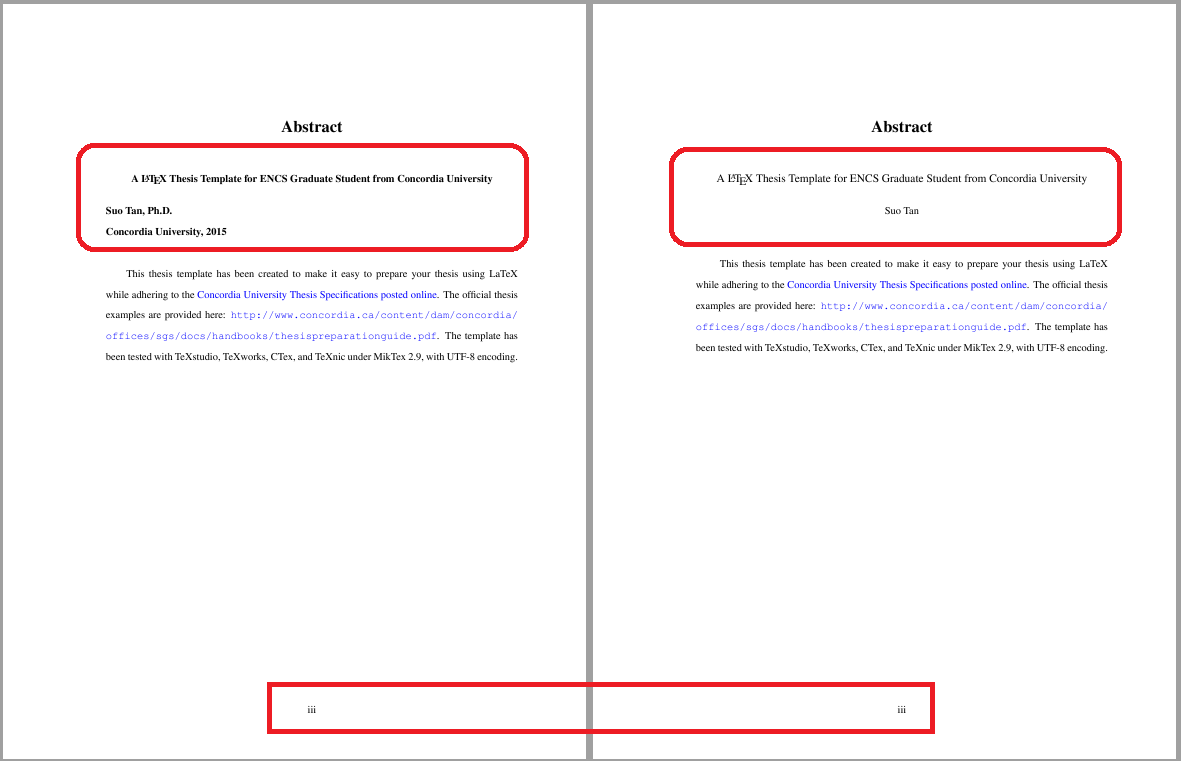
\includegraphics[scale=0.6]{Compare}  %it is suggested to using scale to zoom figures without distortion
        \end{center}
        \caption{An illustration of requirement compliance.}
        \label{fig:Compare}
    \end{figure}
%%%%%%%%%%%%%%%% end figure %%%%%%%%%%%%%%%%%%%
    
    
\subsection{Table}  \label{subSec:Table}
    
 Table \ref{table:ROM_elements} illustrates a very complex table with figures in its cells.
 
 \begin{table}[htp]
     \small{
         \caption{Elements defined for the ROM \citep{Zeng:2008}.}
         \begin{center}
             \label{table:ROM_elements}
             \begin{tabular}{p{1.3cm} p{1.8cm} p{2.1cm} p{4.5cm}} \hline \hline
                 \multicolumn {2}{c}{Type} &  Graphic Representation  & \multicolumn {1}{c}{Description} \\\hline
                 \multirow {3}*{Object} & Object & \hfil \raisebox{-0.35cm}{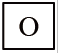
\includegraphics[scale=.5]{FigInTable1_1}} \hfil & Everything in the universe is an object \\
                 & Compound Object & \hfil \raisebox{-0.5cm}{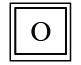
\includegraphics[scale=.5]{FigInTable1_2}} \hfil & It is an object that includes at least two objects in it\\\hline
                 \multirow {7}*{Relation} &  Constraint Relation & \hfil \raisebox{-0.6cm}{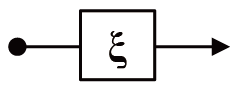
\includegraphics[scale=.4]{FigInTable1_3}} \hfil & It is a descriptive, limiting, or particularizing relation of one object to another\\
                 & Connection & \hfil \raisebox{-0.45cm}{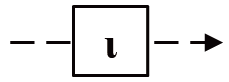
\includegraphics[scale=.4]{FigInTable1_4}} \hfil & It is to connect two objects that do not constrain each other \\
                 & Predicate Relation & \hfil \raisebox{-0.6cm}{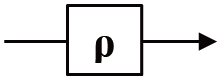
\includegraphics[scale=.4]{FigInTable1_5}} \hfil & It describes an act of an object on another or that describes the states of an object \\\hline \hline
                \end{tabular}
            \end{center}
        }
    \end{table}
    
    
\section{Itemized examples using list structures in \LaTeX{}}
\label{SubSec.:bullet}

Item list using ``\texttt{itemize}" structure are given below:

% itemize style 
\begin{itemize} 
    
    \item  Use bold/italic for emphasis, but keep its use to a minimum. Avoid using underlining in your paper.
    \item  Use a consistent spelling style throughout the paper (US or UK).
    \begin{itemize}  % level 2 items
        \item  Use double quotes.
        \item  Use \%, not percent.
        \item  Do not use ampersands (\&) except as part of the official name of an organization or company.
    \end{itemize}
    \item  Keep hyphenation to a minimum. Do not hyphenate `coordinate' or `non' words, such as `nonlinear'.
    
\end{itemize}

The following are using ``\texttt{enumerate}" structure:

% enumerated style 
\begin{enumerate} 
    
    \item  For complete or near complete sentences, begin with a capital letter and end with a full stop.
    \item  For short phrases, start with lower case letters and end with semicolons.
    
\end{enumerate}

    
\section{Algorithm}
    
    The pseudo code shown in Algorithm \ref{alg:myAlgo} describes the proposed algorithm.
    
    \begin{algorithm}
        \small{
            \caption{Calculate the probability of $G$}\label{alg:myAlgo}
            \begin{algorithmic} [1]
                \Require $p \in [0,1]$, $G$
                \Ensure None
                \For{$i = 0 \to 2^d-1$}\Comment{$d$ is an integer} 
                \If{$n(\nu_i) = 0$}
                \If{ $x < p$}  \Comment{$x$ is a normal distribution number in the range of $[0,1]$}
                \State Occupy $v_i$ site with probability $p$ 
                \EndIf
                \EndIf
                \EndFor
            \end{algorithmic}}
        \end{algorithm}
        
        
  \section{Equation}
        \label{section:equation}
        
        An equation example is shown in Eq. \ref{equ:enc}.
        
        \begin{equation}\label{equ:enc}
        f(ENC)=\int_0^{1}(e^{x}+x^{2})
        \end{equation}
        
\section{Quotations}
        \label{subSec:quotation}
        
        \begin{quote}
            ``It was easier in the beginning when there was only the RED-camera, but now, after RED, it just continuous. And all the different manufacturers, they cannot agree upon what is the standard file format, codec, or compression algorithms, and so on. It is a jungle."
        \end{quote}
        \begin{flushright} CEO, Full Name (Company A) \end{flushright}
        

\section{Citations}
        \label{subSec:Citations}
        
        It is suggested that you choose ``\textbf{$\backslash$citet}" and/or ``\textbf{$\backslash$citep}" to cite references. The ``\textbf{$\backslash$citet\{key\}}" gives you a format of  ``\textbf{Name (1990)}", whileas ``\textbf{$\backslash$citep\{key\}}" delivers a format of ``\textbf{(Name, 1990)}". For example, \citet{Wang&Zeng:2009} extended their research from \citep{Zeng:2008}.
        


        
\chapter{Literature Review} \label{chap:literature}

In this chapter it will be referenced previous literature and related research to this thesis.
It's worth noticing that neural networks have been developed as a medium of defining
problem solving in a defined fashion similar to the structure of the human brain.

Neural networks have emerged as a ubiquitous model in machine learning, due their flexibility 
to adapt to very different types of problems, and handling a numerous amount of variables.
From prediction models to pattern recognition, image processing, or generative models, NN and DL are
techniques that are defined to learn from data, allowing them to do data-driven decisions.
Learning from experience, machines therefore can solve problems without the definition
of a predefined model, but in doing so, at least with a classical implementation, such as
CNN, the definition of the model is then encoded within the a set of neurons, called hidden layer,
makes it more difficult to easily interpret or change the model without re-training the 
neural network with other data that could adapt the output of the model.

For the setup of the neural networks and tools to be used in the implementation
the following components were used:

\subsection{Keras}  \label{subSec:Keras}

Keras is a framework for easy and fast protyping of neural networks 
that can run in CPU or GPU's, excelent for deep learning. It runs using
Python and works as an abstraction layer for another backend suchs as
Tensorflow and Theano. 

Keras contains numerous functions for building blocks such as layers, 
objective functions, activation functions, optimizers, and a set of tools to facilitate 
the work with image and text.

\subsection{Tensorflow}  \label{subSec:Tensorflow}

As defined in their github repository "TensorFlow is an open source software library for numerical computation using data flow graphs.
The graph nodes represent mathematical operations, while the graph edges represent the multidimensional data arrays 
(tensors) that flow between them. This flexible architecture enables you to deploy computation to one or more CPUs or GPUs in a desktop, 
server, or mobile device without rewriting code. TensorFlow also includes TensorBoard, a data visualization toolkit."


%\include{Experiment} % chapter title as the chapter name.


%%%%%%%%%% Appendices %%%%%%%%%%%%%%%%
% ---- Appendix settings. Please Do NOT change them. -----
\appendix
\setcounter{table}{0}		% reset the table counter
\setcounter{figure}{0}		% reset the figure counter
\renewcommand{\thefigure}{\Alph{chapter}.\arabic{figure}} 	% numbering the a figure in Appendix as Figure A.2, Figure B.1, etc.
\renewcommand{\thetable}{\Alph{chapter}.\arabic{table}}		% numbering the a table in Appendix as Table A.2, Table B.1, etc.

%%%%%%%%%% Body of Appendix %%%%%%%%%%%%%%%%
\begin{appendices}
    \chapter{My Appendix} \label{chap:ApdxA}

Appendix figure example is shown in \ref{fig:encslogo} below
 
 %%%%%%%%%%%%%%%% begin figure %%%%%%%%%%%%%%%%%%%
 \begin{figure}[htp]
     \begin{center}
         
\includegraphics[scale=0.5]{ENCSlogo}  %it is suggested to using scale to zoom figures without distortion
        \end{center}
        \caption{An figure example in Appendix \ref{chap:ApdxA}.}
        \label{fig:encslogo}
    \end{figure}
%%%%%%%%%%%%%%%% end figure %%%%%%%%%%%%%%%%%%%
    
    

    %\include{Appendix_B}
\end{appendices}





%%%%%%%%%% References %%%%%%%%%%%%%%%%%
\addcontentsline{toc}{chapter}{Bibliography}  %  Add Bibliography to TOC
\bibliography{ThesisRef}        % Your .bib files name here
\bibliographystyle{apacite}  	% References are in APA style

\end{document}
